\documentclass{beamer}

\usepackage{listings}
\usepackage{color}
\usepackage{hyperref}

\usepackage[T1]{fontenc}
\usepackage{textcomp}
\usepackage{upquote}

% Default fixed font does not support bold face
\DeclareFixedFont{\ttb}{T1}{txtt}{bx}{n}{10} % for bold
\DeclareFixedFont{\ttm}{T1}{txtt}{m}{n}{10}  % for normal

% Custom colors
\usepackage{color}
\definecolor{deepblue}{rgb}{0,0,0.5}
\definecolor{deepred}{rgb}{0.6,0,0}
\definecolor{deepgreen}{rgb}{0,0.5,0}

\usepackage{listings}


% Python style for highlighting
\newcommand\pythonstyle{\lstset{
language=Python,
basicstyle=\ttm,
otherkeywords={self},             % Add keywords here
keywordstyle=\ttb\color{deepblue},
emph={MyClass,__init__},          % Custom highlighting
emphstyle=\ttb\color{deepred},    % Custom highlighting style
stringstyle=\color{deepgreen},
frame=tb,                         % Any extra options here
showstringspaces=false            % 
upquote=True,
columns=fullflexible,
basicstyle=\ttfamily
}}


% Python environment
\lstnewenvironment{code}[1][]
{
%\begin{small}
\pythonstyle
\lstset{#1}
%\end{small}
}
{}


\begin{document}

% numpy theory

\begin{frame}
\frametitle{CS24420 \& MA25220 \& MT25220 \& MX35220 \& CSM0120}

\begin{center}
\begin{huge}
Lecture 7: More NumPy
\end{huge}
\bigskip

Amanda Clare (afc@aber.ac.uk)

\end{center}
\end{frame}


\begin{frame}[fragile]
\frametitle{A tour of some of the functionality of NumPy}
\begin{itemize}
\item Storage
\item Creating ranges
\item Sorting
\item Reading from/writing to files
\end{itemize}
\end{frame}



\begin{frame}[fragile]
\frametitle{NumPy arrays and how they're stored}
NumPy arrays are stored as a linear block of memory (even when they
are multi-dimensional arrays).
\begin{code}
x = np.arange(0, 100)
y = x.reshape((10, 10))
\end{code}
This is how \texttt{y} looks:
\begin{code}
array([[ 0,  1,  2,  3,  4,  5,  6,  7,  8,  9],
       [10, 11, 12, 13, 14, 15, 16, 17, 18, 19],
       [20, 21, 22, 23, 24, 25, 26, 27, 28, 29],
       [30, 31, 32, 33, 34, 35, 36, 37, 38, 39],
       [40, 41, 42, 43, 44, 45, 46, 47, 48, 49],
       [50, 51, 52, 53, 54, 55, 56, 57, 58, 59],
       [60, 61, 62, 63, 64, 65, 66, 67, 68, 69],
       [70, 71, 72, 73, 74, 75, 76, 77, 78, 79],
       [80, 81, 82, 83, 84, 85, 86, 87, 88, 89],
       [90, 91, 92, 93, 94, 95, 96, 97, 98, 99]])
\end{code}
\end{frame}

\begin{frame}[fragile]
\frametitle{NumPy arrays and how they're stored}
\begin{itemize}
\item y is a different view of x
\item Changing an item of y will change the same item in x
\item In memory, it's just a contiguous linear space of elements
\item numpy knows where each row begins in the linear space
\item We could say that a numpy array is just a memory space with an
  indexing method
\item C programmers/Python programmers are used to seeing matrices in row order
\item Fortran programmers are used to column order
\item In numpy you can choose which order you want (order='C' or order='F')
\end{itemize}
\end{frame}

\begin{frame}[fragile]
\frametitle{NumPy arrays and how they're stored}
\begin{itemize}
\item So a numpy array is a linear piece of memory with a way to index it
\item Also with a \texttt{dtype}
\item If you want to change the \texttt{dtype}, then use \texttt{astype}
\end{itemize}
\begin{code}
>>> x = np.arange(0, 10, dtype="int16")
>>> print(x)
array([0, 1, 2, 3, 4, 5, 6, 7, 8, 9], dtype=int16)
>>> y = x.astype("int8")
>>> print(y)
array([0, 1, 2, 3, 4, 5, 6, 7, 8, 9], dtype=int8)
\end{code}
\end{frame}

\begin{frame}[fragile]
\frametitle{NumPy arrays and dtype}
\begin{code}
>>> np.arange(0, 150, dtype='int8')
array([   0,    1,    2,    3,    4,    5,    6,    7,    8,    9,   10,
         11,   12,   13,   14,   15,   16,   17,   18,   19,   20,   21,
         22,   23,   24,   25,   26,   27,   28,   29,   30,   31,   32,
         33,   34,   35,   36,   37,   38,   39,   40,   41,   42,   43, 
         44,   45,   46,   47,   48,   49,   50,   51,   52,   53,   54,
         55,   56,   57,   58,   59,   60,   61,   62,   63,   64,   65,
         66,   67,   68,   69,   70,   71,   72,   73,   74,   75,   76,
         77,   78,   79,   80,   81,   82,   83,   84,   85,   86,   87,
         88,   89,   90,   91,   92,   93,   94,   95,   96,   97,   98,
         99,  100,  101,  102,  103,  104,  105,  106,  107,  108,  
        109, 110,  111,  112,  113,  114,  115,  116,  117,  118,  
        119,  120, 121,  122,  123,  124,  125,  126,  127, -128, 
       -127, -126, -125, -124, -123, -122, -121, -120, -119, 
       -118, -117, -116, -115, -114, -113, -112, -111, -110, 
       -109, -108, -107], dtype=int8)
\end{code}
\end{frame}


\begin{frame}[fragile]
\frametitle{linspace and arange}
\begin{itemize}
\item \texttt{arange} is the equivalent of \texttt{range}
\item \texttt{linspace} will allow \texttt{num} values between start
  and stop, where \texttt{num} defaults to 50
\end{itemize}
\begin{code}
>>> a = np.linspace(0, 10, dtype="int")
>>> print(a)
array([ 0,  0,  0,  0,  0,  1,  1,  1,  1,  1,  2,  2,  2,  2,  2,  3, 
        3,  3,  3,  3,  4,  4,  4,  4,  4,  5,  5,  5,  5,  5,  6,  6, 
        6, 6, 6,  7,  7,  7,  7,  7,  8,  8,  8,  8,  8,  9,  9,  
        9, 9, 10])
>>> b = np.linspace(0, 10, num=7, dtype="int")
>>> print(b)
array([ 0,  1,  3,  5,  6,  8, 10])
>>> c = np.linspace(0, 10, num=7)
>>> print(c)
array([  0. ,  1.66666667, 3.33333333,  5.   ,
         6.66666667,   8.33333333,  10.  ])
\end{code}
\end{frame}

\begin{frame}[fragile]
\frametitle{linspace and arange}
\begin{itemize}
\item Just be careful with floating point numbers
\item They have limited precision and can sometimes be different to
  the answer you expected
\item What is 0.3/3 ? Is it 0.1?
\item 0.09999999999999999
\item For two arrays \texttt{a} and \texttt{b}, you can check if they have the 'same'
  numbers with np.allclose(a,b) or np.isclose(a,b)
\item Other parameters to these functions allow you to set how close is good enough, if
  you don't like the default.
\end{itemize}
\end{frame}


\begin{frame}[fragile]
\frametitle{Sorting numpy arrays in place}
\begin{code}
>>> a = np.array([[4,3,5],[8,7,6],[1,2,3]]) 
>>> a.sort()
>>> print(a)
array([[3, 4, 5],
       [6, 7, 8],
       [1, 2, 3]])
\end{code}
\end{frame}

\begin{frame}[fragile]
\frametitle{Making a sorted copy}
\begin{code}
>>> a = np.array([[4,3,5],[8,7,6],[1,2,3]])
>>> b = np.sort(a)
>>> print(a)
array([[4, 3, 5],
       [8, 7, 6],
       [1, 2, 3]])
>>> print(b)
array([[3, 4, 5],
       [6, 7, 8],
       [1, 2, 3]])
\end{code}
\end{frame}

\begin{frame}[fragile]
\frametitle{{Sorting column-wise}}
\begin{code}
>>> a = np.array([[3,4,5],[6,7,8],[1,9,9]])
>>> print(a)
array([[3, 4, 5],
       [6, 7, 8],
       [1, 9, 9]])
>>> a.sort(axis=0)
>>> print(a)
array([[1, 4, 5],
       [3, 7, 8],
       [6, 9, 9]])
\end{code}
\end{frame}

\begin{frame}[fragile]
\frametitle{{Sort on a column}}
Sort on column 1 (the second column):
\begin{code}
>>> a = np.array([[4,3,5],[8,7,6],[1,2,3]])
>>> print(a[:, 1])
array([3, 7, 2])
>>> b = a[:, 1].argsort()
>>> print(b)
array([2, 0, 1])
>>> print(a[ b ])
array([[1, 2, 3],
       [4, 3, 5],
       [8, 7, 6]])
\end{code}
\end{frame}

\begin{frame}[fragile]
\frametitle{Matrix operations}

foo
\end{frame}

%For example: 
% matrix ops (add, subtract, multiply? multiply is maybe too hard for CS and would need a motivating concept. I toyed with transitive closure as a way of finding flights between cities, but we'd have to work in boolean space so even more hard - np.logical_or(b, np.dot(b,b)). 
% transpose
% normalise a matrix 

\begin{frame}[fragile]
\frametitle{Histograms example}
Swansea measles outbreak 2013:
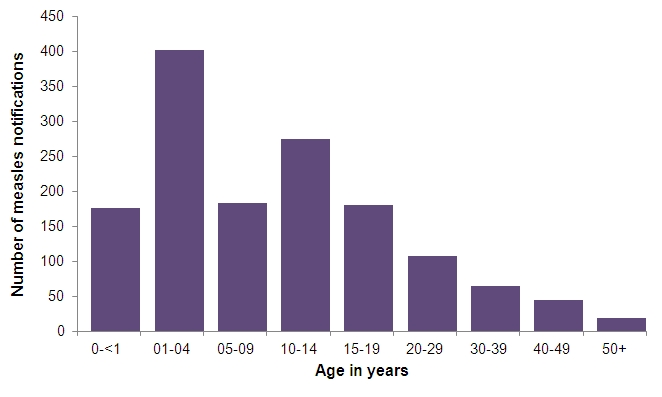
\includegraphics[width=10cm]{measlesbyage01072013.jpg}

Figure taken from Public Health Wales: \url{http://www.wales.nhs.uk/sitesplus/888/page/66389}
\end{frame}


\begin{frame}[fragile]
\frametitle{Histograms}
\begin{code}
>>> m_ages = np.array(
      [13,4,2,11,12,6,13,14,25,16,22,1,8])
>>> np.histogram(m_ages, bins=range(0,35,5))
(array([3,2,5,1,1,1]), array([0,5,10,15,20,25,30]))
\end{code}

Notice that the result is a tuple of two arrays. So we could save these arrays into variables.
\end{frame}

\begin{frame}[fragile]
\frametitle{Histograms}
\begin{code}
>>> m_ages = np.array(
      [13,4,2,11,12,6,13,14,25,16,22,1,8])
>>> (hist,edges) = np.histogram(m_ages,bins=range(0,35,5))

>>> print(hist)
array([3, 2, 5, 1, 1, 1])

>>> print(edges)
array([ 0,  5, 10, 15, 20, 25, 30])
\end{code}

Notice that there is one more element in the \texttt{edges} than in the \texttt{hist}: the \texttt{edges} array includes both the top and bottom edges of the bins.
\end{frame}


\begin{frame}[fragile]
\frametitle{Functions for reading/writing data from files}
\begin{itemize}
\item For reading a file of whitespace or comma separated values: \texttt{loadtxt}
\item Can specify the separator, whether to skip some header lines,
  whether to ignore some columns.
\item \texttt{genfromtxt} if you have missing values or missing lines
\item For writing your aray out to a file: \texttt{savetxt}
\item Can specify delimiter, header, footer.
\item For reading from binary file: \texttt{fromfile}
\end{itemize}
\end{frame}

\begin{frame}[fragile]
\frametitle{loadtxt examples}
\begin{code}
# choose comma delimiters
mydata = np.loadtxt("myfile.csv", delimiter=",")

# enforce loading as integers, not floats
int_data = np.loadtxt("myfile.txt", dtype = int)

# skip a line of header info
data_no_header = np.loadtxt("myfile.tsv", skiprows = 1)
\end{code}
\end{frame}

\begin{frame}[fragile]
\frametitle{Reading binary data}
\begin{itemize}
\item By 'binary' data, we just mean non-text data. 
\item This could be ints or floats.
\item An int is usually stored using 4 bytes (or 32 bits).
\item This means we could just write out 32 bits, then another 32
  bits, then another, and so on.
\item We then know how to read these back in, one after another.
\item But you wouldn't be able to just open this file in, say, Notepad and see
  the ints. It can't guess the format.
\item A float could also be stored using 32 bits (though probably
  64). We might have written out floats instead.
\end{itemize}
\end{frame}

\begin{frame}[fragile]
\frametitle{Reading binary data with fromfile}
\begin{code}
a = np.fromfile("megt90n000cb.img", dtype=np.uint16)
\end{code}
\end{frame}

\begin{frame}[fragile]
\frametitle{Reading the Mars data}
\begin{code}
import numpy as np
import matplotlib.pyplot as plt

# Data file obtained from 
# http://pds-geosciences.wustl.edu/missions/mgs/megdr.html

# Read the data from the file as a 1-dimensional array of 16-bit ints
a = np.fromfile("megt90n000cb.img", dtype=np.uint16)
# Reshape the array to have rows and columns
b = a.reshape(720, 1440)
print(b)
\end{code}
\end{frame}


\begin{frame}[fragile]
\frametitle{Plotting the Mars data}
\begin{code}
# rescale to between 0.0 - 1.0 for plotting with imshow
c = b / 65535.0
# choose a red colourmap, because it's Mars!
plt.imshow(c, cmap="hot")
plt.colorbar()

# If not plotting inline in iPython
plt.show()
\end{code}
\end{frame}




% 4d matrices eg x y z over time

% 4D min max row for each row in each dimension

\end{document}
